\section{Praktkumsaufgabe 7)}
\subsection{Teilaufgabe A)}
\textbf{Entwickeln Sie ein Programm, das einen Aufrufparameter n erwartet und eine initiale n-
tps-Datenbank auf dem gewählten Datenbankmanagementsystem erzeugt.}

Um überhaupt mit der Datenbank zu interagieren mussten wir uns erstmal den
JDBC-Treiber für unser DBMS Postgresql besorgen.

Diesen haben wir anschließend in das Projekt eingebunden und haben mit der
Klasse \gqq{DatabaseConnection} diesen Treiber in der
\gqq{getConnection}-Methode laden lassen.


\lstset{language=Java, backgroundcolor=\color{editorGray},
  basicstyle={\linespread{0.82}\footnotesize\ttfamily},   
  frame=b, xleftmargin={0.75cm},literate=
    {Ö}{{\"O}}1
  {Ä}{{\"A}}1
  {Ü}{{\"U}}1
  {ß}{{\ss}}2
  {ü}{{\"u}}1
  {ä}{{\"a}}1
  {ö}{{\"o}}1,
    numberstyle=\tiny\noncopynumber,
      columns=flexible,
      }
\begin{lstlisting}
	/**
	 * List die Informatioen aus dem Objekt ci (ConnectionInformation) und versucht eine Verbindung 
	 * zur Datenbank auf zu bauen.
	 * 
	 * @throws SQLException Wird geworfen, wenn der DriverManager keine Verbndung zur Datenbank aufbauen kann
	 */
	public void connect() throws SQLException
	{
		/*
		 * Der Compiler uebersetzt " + var + " automatisch in ein StringBuilder Objekt
		 */
		databaseLink = DriverManager.getConnection(
				"jdbc:postgresql://" + ci.getHost() +"/" + ci.getDatabase(),
				ci.getUser(), 
				ci.getPassword()
		);
	}
\end{lstlisting}


Anschließend haben wir eine Klasse \gqq{tpsCreator} implementiert, welche die
gesamte Funktionalität zum Erstellen der \textbf{n-tps-Datenbank} beinhaltet.
Diese Klasse kann man wiederum ein \textit{DatabaseConnection}-Objekt übergeben.
So ist es Möglich in einem Programm mehrere die Datenbank auf verschiedene
Servern anzulegen. Die Verbindungsinformationen übergeben wir mit der Klasse
\nameref{lst:civ1}.

Der Quelltext von tpsCreator befindet sich im Anhang~\nameref{lst:tpsv1}

Als nächstes haben wir uns um die Benutzerinteraktion gekümmert. Wir waren uns
einig, dass wir anstatt auf eine komplexe GUI Darstellung auf eine simple
Konsolen-Anwendung beschränken wollen. Außerdem hat das große Vorteile gegenüer
der Performance.

Um die Interaktion mit der Konsole so einfach wie Möglich zu gestalten haben wir
uns eine Helfer Klasse ~\nameref{lst:crv1} geschrieben und diese anschließend
in unserer \nameref{lst:mainv1} benutzt.
\clearpage

\begin{lstlisting}
			System.out.println("Verbindungsinformationen eingeben!");
			
			System.out.println("Host:");
			infos.setHost(ConsoleReader.readString());

			System.out.println("Datenbank:");
			infos.setDatabase(ConsoleReader.readString());
			
			System.out.println("Benutzer:");
			infos.setUser(ConsoleReader.readString());
			
			System.out.println("Password:");
			infos.setPassword(ConsoleReader.readString());
\end{lstlisting}

Am Ende unserer Main rufen wir die Funkion autoSetup auf. Diese erstellt uns
anschliessend die Datenbank.

\subsection{Teilaufgabe B)}
\textbf{Welche Mindestgrößen schätzen Sie für eine 1-tps-Datenbank bzw. allgemein für eine n-
tps-Datenbank? Wie viel Plattenplatz wird auf dem Datenbank-Server tatsächlich für die
erstellten Datenbanken benötigt?}

Die reine Spaltenanzahl lässt sich folgendermaßen ausrechnen:
\begin{eqnarray}
n + n \cdot 10 + n \cdot 10000
\end{eqnarray}

Also sind bei einer 1-tps-Datenbank 10011 Datensätze enthalten.

Die physikalische Beträgt dabei: 17932460 Bytes. \newline
Umgerechnet ist die Datenbank dementsprechend 17 MB groß.

\subsection{Teilaufgabe C)}
\textbf{Versuchen Sie, die Laufzeit Ihres Programms zu beschleunigen! Dokumentieren Sie
einzelne Verbesserungsideen und die jeweiligen Laufzeitveränderungen für eine lokale
Ausführung Ihres Programms bei der Erzeugung einer 10-tps-Datenbank!}

\subsubsection{Transaction}
Um den Durchsatz der Daten zu erhöhen lassen sich die Queries in einer
Transaction zusammenfassen.  

Dazu muss die Option \textit{autoCommit} abgeschaltet werden und die Transaktion
mit einem manuellen \textit{commit} zum Server geschickt werden. Wir müssen also
unseren \nameref{lst:tpsv1} erweitern. Dafür legen wir 2 neue Funktionen an und
erweitern nebenbei die anderen Funktionen um ein zuschaltbares Debug-Logging.


\clearpage
\begin{lstlisting}
	public void beginTransaktion() {
		try {
			connection.databaseLink.setAutoCommit(false);
		} catch (SQLException e) {
			e.printStackTrace();
		}
	}
	
	public void endAndCommitTransaction() {
		try {
			connection.databaseLink.commit();
			connection.databaseLink.setAutoCommit(true);
		} catch (SQLException e) {
			e.printStackTrace();
		}
	}
\end{lstlisting}


Jetzt brauchen wir noch die funktionalität, um die Funktionen zu benutzen. Damit
wir recht flexibel sind implentieren wir hierfür ein Konsolen-Menü. Dieses
erstellt uns dann eine Benchmark Klasse die die tpsCreator-Klasse alle nötigen
Parameter übergibt und das Benchmarking ausführt.\\

\begin{lstlisting}

	public static int renderMenu() {
		System.out.println("======================- Benchmark Menu -===========================");
		System.out.println("= Wähle bitte eine der folgende Optionen:                         =");
		System.out.println("= (1) Benchmark, Debug Log, incl. drop & create                   =");
		System.out.println("= (2) Benchmark, Debug Log, excl. drop & create                   =");
		System.out.println("= (3) Benchmark, Debug Log, transactions, incl. drop & create     =");
		System.out.println("= (4) Benchmark, Debug Log, transactions, excl. drop & create     =");
		System.out.println("= (5) Benchmark, incl. drop & create                              =");
		System.out.println("= (6) Benchmark, excl. drop & create                              =");
		System.out.println("= (7) Benchmark, transactions, incl. drop & create                =");
		System.out.println("= (8) Benchmark, transactions, excl. drop & create                =");
		System.out.println("===================================================================");
		System.out.print("= Auswahl: ");
		
		return ConsoleReader.readInt();
	}
\end{lstlisting}

 
Die Queries, die mittels einer Transaktion übertragen worden sind, sind bei
einer 1-tps-Datenbank um \ca das 11fache schneller als die Queries die einzelnt
zum Server geschcikt worden sind.

\begin{figure}[!htbp] 
    \subfigure[mit
    Transactions]{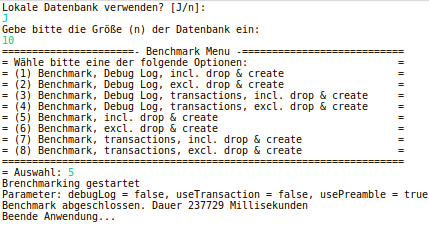
\includegraphics[width=0.49\textwidth]{Bilder/Auswahl_014.png}}
    \subfigure[ohne
    Transaction]{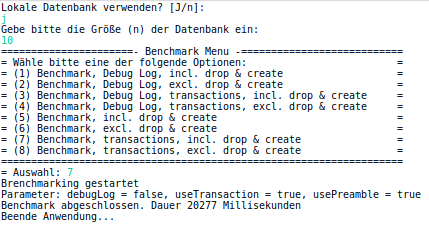
\includegraphics[width=0.49\textwidth]{Bilder/Auswahl_015.png}}
\end{figure} 


\subsubsection{Prepared Statements}
Selbst in einer Transaktion wird jeder einzelne Query validiert. Wir besitzen
aber eine Maße von gleich strukturierten Statements,  Jeden einzelnen zu
validieren kostet den Server Zeit und Ressourcen.
 
 Wir suchen also eine Möglichkeit eine vorher definierte und validierte Struktur
 eines Queries zu bekommen. Dazu bietet sich das \textbf{Prepared Statement} an.
 Wie der Name schon sagt, wird dieser Query einmal zum Server geschickt und
 validiert. Anschließend kann man mit der Reference des Prepared Statements
 schnell und sicher die Daten dem Server übergeben.
 
Die umgeschriebene Funktion für Accounts sieht nun folgendermaßen aus:
 \begin{lstlisting}

	public boolean createAccountTupel(int n) {
		int localConst = n*10000;
		int localRandom;		
		try {
			PreparedStatement insertBranches = connection.databaseLink.prepareStatement("INSERT INTO accounts (accid, NAME, balance, address, branchid) VALUES(?, 'account', 0,'test', ?)");
			
			for (int i = 1; i <= localConst; i++) {
				localRandom = ThreadLocalRandom.current().nextInt(1, n + 1);
				insertBranches.setInt(1, i);
				insertBranches.setInt(2, localRandom);
				insertBranches.addBatch();
				
				if(isDebug) {
					System.out.println("INSERT INTO branches (branchid, branchname, balance,address) VALUES(" + i + ", 'branch', 0, 'branch')"); }
			}

			insertBranches.executeBatch();
			return true;
		} catch (SQLException e) {
			e.printStackTrace();
		}
		return false;
	}
 \end{lstlisting}

Eine gute Eigenschaft von den Prepared Statements ist, dass sie die
Transaktionsverwaltung schon intregriert haben und damit bei gleichen Queries
deutlich schneller sind als ein normales Statement, welches ein und den selben
Query immer und immer wieder ausführt. Diese Eigenschaft besitzt ein
Prepared Statement auch, wenn das Feature \textit{autoCommit} aktiviert ist.

Um aber aussagekräftige Benchmarks zu erhalten, ist gerade das Feature
hinderlich, Wir möchten ja die Queries auch ohne Transaktion ausführen können,
deshalb müssen wir uns eine alte Kopie der Klasse behalten und bei Bedarf
instanziieren.
\begin{center}
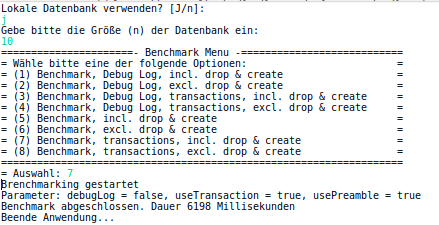
\includegraphics{Bilder/Auswahl_016.png}
\end{center}
Mit den Prepared Statement ist unser Benchmark jetzt \textbf{36fach} schneller
als unser ursprüngliches Benchmark Tool.

\subsubsection{Adressauflösung von Domainnamen}
Um das Ergebniss noch mehr zu verbessern kommt jetzt das Feintuning. Dazu
schauen wir uns jetzt nicht das DBMS an, sondern DNS-Server.

Hier besteht ein massiver Nachteil gegenüber der herkömmlicher IP. Jeder
DNS-Server \bzw DNS-Cache muss in irgendeiner Tabelle nachschauen, welche Domain
zu welcher IP gehört. 

Selbst der lokale DNS-Cache muss dies \zB für \textbf{localhost} machen.
Zugriffe bedeuten bekanntlich Zeit. Möchten wir also diese Zugriffszeiten
umgehen, brauchen wir einfach nur die IP-Adresse statt des Domainnamens
einzugeben. Dies wäre für \textbf{localhost} entweder \gqq{127.0.0.1} als
IPv4-Schreibweiße oder \gqq{[::1]} als IPv6 Schreibweise.

\subsubsection{IDs vom Server generieren lassen}
-- bis hierher bin ich gekommen .- lg mario
ps: habe nicht auf rächtschreibung geachtet, habe einfach mal drauf los getippz,
vieles ist noch überarbeitungswürdig

\subsection{Teilaufgabe D)}
\textbf{Messen und protokollieren Sie die Laufzeit ihres optimierten Programms für n=10, n=20
und n=50 sowohl lokal auf dem Datenbank-Server als auch von einem "remote" Client!
(Gemessen werden soll nur die Laufzeit zum Einfügen ohne evtl. notwendige vorherige
DROP-TABLE- oder CREATE-TABLE-Anweisungen!)}

